\documentclass[11pt]{article}
\usepackage[margin=1in]{geometry}
\usepackage{amsmath,amssymb,amsthm}
\usepackage{booktabs,tabularx,array}
\usepackage{graphicx}
\usepackage{enumitem}
\usepackage[hidelinks]{hyperref}
\usepackage{xcolor}
\providecommand{\euro}{\texteuro}

\newtheorem{proposition}{Proposition}
\newtheorem{lemma}{Lemma}
\theoremstyle{definition}
\newtheorem{assumption}{Assumption}
\newtheorem{remark}{Remark}

\newcommand{\ybar}{\bar y}
\newcommand{\Dz}{\Delta^{0}}
\graphicspath{{../output/model_step1/}}
\setlist{itemsep=2pt,topsep=4pt}

\title{Step 1: A competitive two-season benchmark\\for storage under a fill mandate}
\author{Working notes}
\date{November 2026}

\begin{document}
\maketitle

\begin{abstract}
\noindent This note sets up and solves the first building block of the storage model: a
deterministic summer/winter market in which storage moves prices in both seasons, storers
are competitive, and the regulator imposes a minimum fill level before winter. Everything is
closed form. The block isolates the \emph{cost side} of a mandate: with complete markets and no
security externality, a binding mandate can only lower total welfare. It also delivers objects
that later steps need: the shadow cost of the target (in \euro/MWh), its incidence across
summer consumers, winter consumers, importers, storers and taxpayers, the crowding out of
private storage by state filling, and an estimable equation linking the seasonal spread to the
level of fill. The security-of-supply benefit is added in Step 2 and is priced against exactly
the shadow cost derived here.
\end{abstract}

\section{Purpose and what is deliberately left out}

The research question is how to regulate storage for security of supply at least welfare cost.
Step 1 answers a narrower question that the full model needs as an input:
\emph{if security of supply were not at stake, what would a fill mandate cost, who would pay,
and through which channel?} The channel is the seasonal price spread: a mandate forces more
injection than the market would choose, which raises summer prices, lowers winter prices and
compresses the spread that pays for storage. The spread is the mechanism; the objects of interest
are fill on 1 November, the welfare cost, and its distribution.

The benchmark keeps the ingredients that make storage regulation non-trivial and that survive into
the structural model:
\begin{enumerate}
\item \textbf{Endogenous prices in both seasons.} Storage demand in summer and storage supply in
winter shift the price, with import supply (LNG and pipeline) upward sloping. This nests the
price-taking environment of Ejarque (2011) as the limit of perfectly elastic imports.
\item \textbf{A merit order of storage facilities.} Facilities differ in cost (salt caverns,
depleted fields, aquifers; injection ratchets). This gives an upward-sloping aggregate storage cost
and inframarginal rents, which matter for how a mandate is financed.
\item \textbf{Capacity and injection limits}, discounting, and a target defined relative to capacity
(or to consumption), as in the EU regulation.
\end{enumerate}
It leaves out uncertainty (Step 2), market power in storage (Step 3), the injection path inside the
summer and the 1 November deadline (Step 4), and monthly dynamics, several countries and calibration
(Step 5). Section~\ref{sec:extensions} says how each piece plugs into the formulas below.

\section{Environment}

\subsection{Seasons, demand and import supply}
There are two seasons, summer $t=1$ (April--September) and winter $t=2$ (October--March).
Quantities are TWh per season and prices \euro/MWh. In each season final demand is linear,
\begin{equation}
P_t = A_t - b_t D_t, \qquad b_t>0,
\end{equation}
where $A_t$ collects heating and cooling degree days, gas-for-power demand and industrial activity.
Gas comes from imports and domestic production with an upward-sloping supply,
\begin{equation}
P_t = a_t + g_t M_t, \qquad g_t\ge 0.
\end{equation}
A flat $g_t=0$ is a perfectly elastic world LNG market; a steep $g_t$ captures binding regasification
or pipeline capacity and competition with Asian buyers. Seasonal slopes are allowed to differ:
winter heating demand is less elastic than summer power-sector demand ($b_2$ vs $b_1$), and import
capacity is tighter in winter ($g_2$ vs $g_1$).

\subsection{Storage}
Storers inject $y$ in summer and withdraw it in winter. Market clearing is
\begin{equation}
M_1 = D_1 + y, \qquad M_2 + y = D_2 .
\end{equation}
Aggregate storage cost is
\begin{equation}
C(y) = c\,y + \tfrac{\kappa}{2}y^{2}, \qquad 0\le y \le K,
\end{equation}
with $c$ the unit injection, withdrawal and fuel cost of the cheapest facilities and $\kappa\ge 0$ the
slope of the facility merit order: if facilities are ranked by unit cost and spread uniformly
from $c$ to $c+\kappa K$, the marginal cost of storing the $y$-th unit is $c+\kappa y$. $K$ is
\emph{effective} capacity, $K=\min\{\text{working gas volume},\ \text{injection rate}\times
\text{injection days}\}$; in two periods an injection-rate limit is just a tighter capacity (it bites
separately only once the summer is split, Step 4). The capacity itself is sunk in Step 1.
Winter revenue is discounted with $\beta\in(0,1]$ (half-year).

\begin{remark}[Initial stock]
If storage enters the summer holding $x_0$ (cushion gas excluded), replace $K$ by $K-x_0$ and the
target $\theta K$ by $\theta K-x_0$ below. A low end-of-winter stock (as in spring 2022) tightens the
mandate one-for-one.
\end{remark}

\subsection{Residual price functions}
Solving demand and supply for given $y$ gives the summer and winter prices as linear functions of
storage. Define, for each season,
\begin{equation}
s_t \equiv \frac{b_t g_t}{b_t+g_t}, \qquad
\omega_t \equiv \frac{g_t}{b_t+g_t}\in[0,1],\qquad
P^0_t \equiv \frac{g_tA_t+b_ta_t}{b_t+g_t}, \qquad D^0_t\equiv \frac{A_t-a_t}{b_t+g_t}.
\end{equation}
$P^0_t$ and $D^0_t$ are the no-storage price and quantity; $s_t$ is the price impact of one TWh of
storage; $\omega_t$ is the share of a storage change absorbed by consumption, and $1-\omega_t$ the
share absorbed by imports.

\begin{lemma}[Prices and quantities]\label{lem:prices}
For given storage $y$ (with imports interior, Assumption~\ref{ass:interior}),
\begin{align}
P_1(y) &= P^0_1 + s_1 y, & D_1(y) &= D^0_1-\omega_1 y, & M_1(y) &= D^0_1+(1-\omega_1)y,\\
P_2(y) &= P^0_2 - s_2 y, & D_2(y) &= D^0_2+\omega_2 y, & M_2(y) &= D^0_2-(1-\omega_2)y.
\end{align}
\end{lemma}

\begin{assumption}\label{ass:interior}
Imports are positive in both seasons, $M_2(y)>0$ for all $y\le K$: imports stay the marginal source
in winter. (This holds for the EU after 2022; otherwise the winter price function kinks at the point
where storage alone serves demand.)
\end{assumption}

Two composite slopes recur throughout:
\begin{equation}
\sigma \equiv s_1 + \beta s_2, \qquad \Lambda \equiv \sigma+\kappa .
\end{equation}
$\sigma$ is how fast storage compresses the discounted seasonal spread; $\Lambda$ adds the rising
marginal cost of storage. Finally, the \emph{no-storage net spread} is
\begin{equation}
\Dz \equiv \beta P^0_2 - P^0_1 - c,
\end{equation}
the margin the first (cheapest) unit of storage would earn. It is the single index of seasonality in
the model: anything that raises winter demand relative to summer demand raises $\Dz$.

\section{Competitive equilibrium}

Storers are price takers. Facility owners choose $y$ to maximise
$\Pi(y)=\left(\beta P_2-P_1-c\right)y-\frac{\kappa}{2}y^{2}$ at given prices, subject to $0\le y\le K$.
Equivalently, the marginal facility stores if and only if the discounted spread covers its cost.

\begin{proposition}[Equilibrium]\label{prop:eq}
The competitive storage level is
\begin{equation}
y^{*}=\min\left\{K,\ \max\left\{0,\ \frac{\Dz}{\Lambda}\right\}\right\},
\end{equation}
with prices $P_1^*=P_1^0+s_1y^*$ and $P_2^*=P_2^0-s_2y^*$. At an interior $y^*$ the arbitrage
condition holds with the marginal facility's cost:
\begin{equation}
\beta P_2^* - P_1^* = c + \kappa y^*,
\end{equation}
storers earn inframarginal rents $\Pi(y^*)=\frac{\kappa}{2}y^{*2}$, and if $y^*=K$ capacity earns a
scarcity rent $\mu=\Dz-\Lambda K\ge 0$ per unit.
\end{proposition}

\paragraph{Comparative statics of $y^*$ (interior).}
$y^*$ rises with seasonality ($\Dz$: higher $A_2$, lower $A_1$) and with $\beta$, and falls with $c$,
$\kappa$, and the price impacts $s_1,s_2$. With perfectly elastic imports ($s_1=s_2=0$) storage moves no
price, $y^*=\Dz/\kappa$, and with $\kappa=0$ the problem becomes bang-bang ($y^*\in\{0,K\}$): this is the
exogenous-price world of Ejarque (2011), where only a penalty or reserve rule can generate interior
choices. The endogenous-price model makes the private choice interior and continuous in primitives,
which is what we need to price a mandate.

\begin{proposition}[Efficiency]\label{prop:eff}
Let total surplus be $W(y)=\sum_t\beta^{t-1}\left[CS_t(y)+PS_t(y)\right]+\Pi(y)$, i.e.\ consumers,
importers and storers, with lump-sum transfers netting out. Then
\begin{equation}
W'(y)=\beta P_2(y)-P_1(y)-c-\kappa y=\Dz-\Lambda y, \qquad W''(y)=-\Lambda<0,
\end{equation}
so $y^*$ maximises $W$ on $[0,K]$. With complete markets and no externality, the competitive fill is
efficient and any binding mandate lowers total welfare.
\end{proposition}

This is the benchmark against which every later market failure (Step 2) and market-power
distortion (Step 3) is measured. Section~\ref{sec:whose} shows one exception that already arises in
Step 1, when the welfare of foreign gas suppliers is not counted.

\section{The fill mandate}

The regulation requires storage to be at least a share $\theta$ of capacity before winter:
\begin{equation}
y \ \ge\ \ybar \equiv \min\{\theta K,\ \phi\,\bar D\},
\end{equation}
with $\theta=0.9$ in the EU regulation, and $\phi\bar D$ the cap at a share of average annual consumption
($\phi=0.35$ in the regulation), which bites in countries with storage large relative to demand. More
flexible versions of the rule (a window around the deadline, permitted deviations in adverse market
conditions) act in this model as a lower effective $\theta$. Write the \emph{mandate gap}
$G\equiv\ybar-y^*$.

\begin{proposition}[Regimes]\label{prop:regimes}
Suppose $0<y^*<K$. With an unfunded hard mandate, equilibrium storage is $\max\{y^*,\ybar\}$, and there are
three regimes:
\begin{enumerate}[label=(\roman*)]
\item \textbf{Non-binding}, $\Dz \ge \Lambda\ybar$: the market fills above the target; nothing changes.
\item \textbf{Binding, storers still profitable}, $(\sigma+\tfrac{\kappa}{2})\ybar \le \Dz < \Lambda\ybar$:
the marginal units lose money, but inframarginal rents cover the losses, $\Pi(\ybar)\ge 0$.
\item \textbf{Binding, storers loss-making}, $\Dz < (\sigma+\tfrac{\kappa}{2})\ybar$: $\Pi(\ybar)<0$, so the
mandate is not individually rational without compensation.
\end{enumerate}
Inside regime (iii), the spread itself inverts ($\beta P_2<P_1$) when $\sigma\ybar>\Dz+c$, i.e.\ when the gap
exceeds $G>(c+\kappa y^*)/\sigma$.
\end{proposition}

The thresholds are linear in $\ybar=\theta K$. Holding seasonality fixed, a country is more likely to
be in regimes (ii)--(iii) the larger its storage relative to its seasonal swing, which is why the
consumption cap $\phi\bar D$ exists. An inverted summer--winter spread, which is often read as a
market signal, can in this model be the mandate's own footprint.

\section{Price, spread and quantity effects}

\begin{proposition}[Effects of a binding mandate]\label{prop:effects}
Relative to the competitive outcome, a binding mandate changes
\begin{align}
\Delta P_1 &= s_1 G, \qquad \Delta P_2 = -s_2G, \qquad
\Delta(\beta P_2-P_1) = -\sigma G,\\
\Delta D_1 &= -\omega_1 G, \quad \Delta M_1 = (1-\omega_1)G, \qquad
\Delta D_2 = \omega_2 G, \quad \Delta M_2 = -(1-\omega_2)G .
\end{align}
The shadow cost of the target, the multiplier on $y\ge\ybar$, is
\begin{equation}
\nu = \Lambda G \quad(\text{\euro/MWh}),
\end{equation}
the loss on the last mandated MWh. It is also the per-unit subsidy that would induce the same fill
voluntarily.
\end{proposition}

Two readings matter for security of supply.
\begin{itemize}
\item \textbf{Where the extra summer gas comes from.} A share $1-\omega_1$ of the extra injection is new
imports and a share $\omega_1$ is summer consumption that is priced out. When summer import supply is tight
($g_1$ large, $\omega_1\to 1$) the mandate is filled by \emph{demand destruction} in summer (industry and
gas-fired power), not by more LNG.
\item \textbf{Where the extra winter gas goes.} A share $1-\omega_2$ of the extra withdrawal \emph{displaces
winter imports} and only $\omega_2$ raises winter consumption. With elastic winter imports, mandated
storage mostly substitutes for imports that would have arrived anyway. In a deterministic world that is
all it does; its security value is that it replaces imports \emph{that might not arrive}, which is exactly
the state that Step 2 adds. The product $(1-\omega_2)G$ is the reduction in winter import dependence
bought by the mandate.
\end{itemize}

\section{Welfare and incidence}\label{sec:welfare}

\begin{proposition}[Deadweight loss and incidence]\label{prop:dwl}
For $0<y^*<\ybar\le K$ the deadweight loss of an unfunded mandate is exact and quadratic in the gap:
\begin{equation}
\text{DWL} = W(y^*)-W(\ybar)=\tfrac{1}{2}\Lambda G^{2}=\tfrac{1}{2}\nu G .
\end{equation}
If the market would not store at all ($\Dz\le 0$, $y^*=0$), $\text{DWL}=\frac12\Lambda\ybar^2+|\Dz|\ybar$.
The DWL is the net of the following transfers (exact for linear demand and supply; $X^*$ denotes values at $y^*$):
\begin{align}
\Delta CS_1 &= -s_1G\left[D_1^*-\tfrac{\omega_1}{2}G\right] &&\text{(summer consumers, $-$)}\\
\Delta PS_1 &= \phantom{-}s_1G\left[M_1^*+\tfrac{1-\omega_1}{2}G\right] &&\text{(summer importers, $+$)}\\
\beta\Delta CS_2 &= \phantom{-}\beta s_2G\left[D_2^*+\tfrac{\omega_2}{2}G\right] &&\text{(winter consumers, $+$)}\\
\beta\Delta PS_2 &= -\beta s_2G\left[M_2^*-\tfrac{1-\omega_2}{2}G\right] &&\text{(winter importers, $-$)}\\
\Delta \Pi &= -\sigma G\,y^* - \left(\sigma+\tfrac{\kappa}{2}\right)G^{2} &&\text{(storers, $-$)}
\end{align}
\end{proposition}

Three points follow.
\begin{enumerate}
\item \textbf{The welfare cost is second order; the transfers are first order.} DWL is quadratic in $G$;
every transfer is linear in $G$ and scales with market size ($D^*_t$, $M^*_t$, $y^*$). Small mandate gaps
are cheap in efficiency terms but large in distributional terms. This is why the political economy of
mandates is about who pays, and why the financing choice (Section~\ref{sec:financing}) matters as much as
the target.
\item \textbf{Storers lose on all their gas, not only on the extra units.} The term $\sigma G y^*$ is the
spread compression applied to the volume the market would have stored anyway. It is a transfer to winter
consumers. An unfunded mandate therefore taxes storage capacity; in the long run (when $K$ becomes a
choice, Step 5) it erodes the capacity that security of supply relies on.
\item \textbf{Consumers as a whole can gain.} Net consumer surplus changes by
$G\left[\beta s_2D_2^*-s_1D_1^*\right]+\frac{G^2}{2}\left[\beta s_2\omega_2+s_1\omega_1\right]$, positive when
winter consumption is large and winter prices react strongly. Consumer gains then come from storers and
from winter import suppliers.
\end{enumerate}

\subsection{Whose welfare: the terms-of-trade motive}\label{sec:whose}
The EU imports most of its gas, so importer surplus $PS_t$ largely accrues to foreign suppliers. Let a
domestic regulator weigh it by $\alpha\in[0,1]$ ($\alpha=0$: all foreign). Then
$W_\alpha'(y)=\Dz-\Lambda y-(1-\alpha)\left[s_1M_1(y)-\beta s_2M_2(y)\right]$, and
\begin{equation}
y^{\alpha}=\frac{\Dz-(1-\alpha)\left(s_1D_1^0-\beta s_2D_2^0\right)}
{\Lambda+(1-\alpha)\left[s_1(1-\omega_1)+\beta s_2(1-\omega_2)\right]} .
\end{equation}

\begin{proposition}[Domestic optimum]\label{prop:tot}
For $\alpha<1$, $y^\alpha>y^*$ if and only if $\beta s_2M_2^*>s_1M_1^*$: the domestic regulator wants more
storage than the market when winter imports are large and winter import prices are sensitive.
\end{proposition}

Storage shifts import purchases from the season when supply is steep to the season when it is flat, which
lowers the average import bill. Competitive storers do not internalise this pecuniary effect. It is a
genuine rationale for a mandate from a national or EU perspective even without uncertainty, but it is a
transfer from foreign suppliers rather than an efficiency gain, it vanishes with elastic LNG, and between
EU member states it is partly a transfer from neighbours (Step 5).

\section{How the mandate is financed}\label{sec:financing}

The same fill $\ybar$ can be reached in several ways. All the variants below produce the same prices and
the same allocation, hence the same DWL $\frac12\Lambda G^2$, unless stated. They differ in who pays,
in whether private storage is crowded out, and in the additional distortion of raising the money. Let
$\lambda_g\ge 0$ be the marginal cost of public funds.

\begin{enumerate}[label=(\alph*)]
\item \textbf{Unfunded hard mandate} (storers bear it). Incidence as in Proposition~\ref{prop:dwl}; no
public money. Feasible only if storers cannot exit, and it taxes capacity in the long run.

\item \textbf{Per-unit subsidy or premium} $\tau_s$ per MWh stored. Storers choose $y=(\Dz+\tau_s)/\Lambda$,
so $\tau_s=\nu=\Lambda G$. The bill is $\nu\ybar$, and storers end with $\Pi=\frac{\kappa}{2}\ybar^2$, more than
their competitive rent $\frac\kappa2 y^{*2}$: a uniform premium pays every unit at the marginal unit's
loss and so over-compensates inframarginal facilities by $\frac{\kappa}{2}(\ybar^2-y^{*2})$. Extra welfare cost:
$\lambda_g\nu\ybar$.

\item \textbf{Lump-sum compensation} (tender, capacity payment or contract for differences that
tops up the spread to a reference level). Minimum payment to keep storers whole relative to $y^*$:
$T=\Pi(y^*)-\Pi(\ybar)=\Lambda\ybar G-\frac{\kappa}{2}(\ybar^2-y^{*2})$; minimum payment for participation only:
$\max\{0,-\Pi(\ybar)\}$. Cheaper than (b) because it does not pay the marginal premium on inframarginal gas;
the difference is an information rent that a well-designed auction can extract.

\item \textbf{Consumption levy} (as the German storage levy). A levy $\ell$ per MWh of final consumption in
season $t$ lowers the producer price by $\omega_t\ell$, so importers bear a share $\omega_t$; it raises
$\ell D_t$ and adds a Harberger triangle $\frac{1}{2}\ell^2/(b_t+g_t)$. To raise $T$, $\ell\approx T/D_t$, so the
levy's own distortion $\approx\frac12 T^2/[D_t^2(b_t+g_t)]$ is small when the base is broad. A levy only in
winter also lowers the winter producer price and so the spread, feeding back on $y^*$; a year-round levy
on both seasons largely does not. A levy charged on exports moves part of the cost to neighbours (Step 5).

\item \textbf{State filling as buyer of last resort} (a market-area manager or state entity fills the residual).
Private storers anticipate it and respond to the compressed spread, so with facilities used in merit order
\begin{equation}
y_p=\max\left\{0,\ \frac{\Dz-\sigma\ybar}{\kappa}\right\},\qquad z=\ybar-y_p,
\qquad \frac{\partial y_p}{\partial \ybar}=-\frac{\sigma}{\kappa}.
\end{equation}
The state must fill $z=(\Lambda/\kappa)G>G$: each mandated TWh crowds out $\sigma/\kappa$ TWh of private storage.
When the storage merit order is flat relative to price impacts ($\kappa\ll\sigma$) crowding out is close to complete,
and the state ends up holding nearly all the gas. Prices and DWL are as in (a); the state's financial loss is
$\frac{\kappa}{2}z^2$ when $y_p>0$ and $(\sigma\ybar-\Dz)\ybar+\frac\kappa2\ybar^2$ (equal to storers' loss in (a)) when
$y_p=0$.

\item \textbf{Strategic reserve not released in normal winters} (Ejarque's reserve $\lambda$). A volume $R$
bought in summer and held: $P_1$ rises by $s_1R$ but $P_2$ does not fall. Private storage falls by
$s_1R/\Lambda$, less crowding out than (e), but the reserve is a pure cost in Step 1. Its value exists only in the
crisis state of Step 2.

\item \textbf{Soft mandate with a penalty} $k$ per MWh of shortfall (Ejarque's $k(\cdot)$). Storers fill
$y=\min\{\ybar,\ y^*+k/\Lambda\}$: the penalty acts as a cap on the shadow cost, $\nu\le k$, and bounds the DWL by
$k^2/(2\Lambda)$. It turns a quantity rule into a price rule, trading certainty of fill for a ceiling on cost.
\end{enumerate}

\begin{table}[ht]
\centering\small
\begin{tabularx}{\textwidth}{l>{\raggedright\arraybackslash}X>{\raggedright\arraybackslash}X>{\raggedright\arraybackslash}X}
\toprule
Instrument & Who pays & Extra distortion & Crowding out of private storage\\
\midrule
(a) Unfunded mandate & storers ($\Delta\Pi<0$) & long-run capacity exit & none (all storage is private)\\
(b) Per-unit premium & taxpayers, $\nu\ybar$ & $\lambda_g\nu\ybar$; over-compensates rents & none\\
(c) Lump-sum / CfD & taxpayers, $T<\nu\ybar$ & $\lambda_gT$ & none\\
(d) Consumption levy & consumers and importers ($\omega_t$) & $\tfrac12\ell^2/(b_t+g_t)$; base erosion & none; may shift $y^*$ if seasonal\\
(e) State filling & taxpayers, $\tfrac\kappa2z^2$ & $\lambda_g\tfrac\kappa2z^2$ & $\sigma/\kappa$ per mandated TWh\\
(f) Reserve not released & taxpayers, full cost & no winter price relief & $s_1/\Lambda$ per TWh\\
(g) Penalty & storers, up to $k$ per MWh & caps $\nu\le k$ & none; fill uncertain\\
\bottomrule
\end{tabularx}
\caption{Ways to implement the same fill target. Prices, allocation and DWL $\tfrac12\Lambda G^2$ coincide for
(a)--(e); (f) and (g) change the allocation.}
\label{tab:financing}
\end{table}

\section{Comparative statics: when is the mandate expensive?}\label{sec:cs}

All the costs are driven by $G=\ybar-\Dz/\Lambda$ and by $\Lambda$, so the comparative statics are transparent.

\begin{proposition}[Drivers of the cost]\label{prop:cs}
In the binding regime, with $\nu=\Lambda\ybar-\Dz$ and $\text{DWL}=(\Lambda\ybar-\Dz)^2/(2\Lambda)$:
\begin{enumerate}[label=(\roman*)]
\item \textbf{Seasonality.} A higher summer demand shifter $A_1$ (cooling demand, gas-for-power in heatwaves,
low hydro or nuclear availability) raises $P_1^0$ by $\omega_1\,\Delta A_1$, lowers $\Dz$ one-for-one, lowers $y^*$ by
$\omega_1\Delta A_1/\Lambda$, and raises the shadow cost by $\omega_1\Delta A_1$. A milder winter (lower $A_2$, fewer heating
degree days) does the same through $P_2^0$. The DWL is convex in the loss of seasonality.
\item \textbf{Import elasticity.} More elastic imports (lower $s_t$) raise $y^*$ and lower $\Lambda$, so for a given gap
the mandate is cheaper. Tight winter import capacity (high $s_2$) raises $\Lambda$ and the cost of each mandated TWh,
but also the terms-of-trade motive of Proposition~\ref{prop:tot}.
\item \textbf{Capacity.} Since $\ybar=\theta K$, $\partial\nu/\partial K=\Lambda\theta>0$ in the binding regime: countries with
storage large relative to their seasonal swing bear the highest cost per MWh of the target.
\item \textbf{Financing conditions.} A lower $\beta$ (higher interest rates) lowers $\Dz$ and raises the cost of the target.
\end{enumerate}
\end{proposition}

Part (i) connects the model to the ``distorted seasonality'' evidence: anything that narrows the gap between
winter and summer demand turns a non-binding 90\% target into a binding and increasingly costly one, and the
cost rises with the square of the shortfall.

\paragraph{Mapping to data.} Proposition~\ref{prop:effects} gives a reduced form that the data can speak to:
\begin{equation}
\beta P_{2,y}-P_{1,y} \;=\; \underbrace{(\Dz+c)}_{\text{seasonality shifters: HDD, CDD, gas-for-power}} \;-\; \sigma\,\text{Fill}_{y} \;+\; \varepsilon_y ,
\end{equation}
across gas years and countries. $\sigma$ is identified by fill variation that is not driven by the seasonal shifters
themselves (the mandate's introduction in 2022 and its country-specific bite, or initial-stock shocks), and
$\kappa$ comes from facility tariffs and injection ratchets in the facility-level data. $s_1$ and $s_2$ separately follow
from demand and import supply elasticities. These are the parameters Step 5 needs.

\section{Illustration}\label{sec:illustration}

The figures evaluate the formulas on round, EU-sized numbers (code: \texttt{code/model\_step1\_benchmark.R}). They
are an illustration, not a calibration. $K=1{,}100$ TWh; consumption 1{,}300 TWh in summer and 2{,}000 TWh in winter;
demand elasticities 0.20 (summer) and 0.15 (winter); import supply elasticities 1.0 (summer) and 0.8 (winter); storage
unit cost from 1.5 to 5.5 \euro/MWh across the merit order; $\beta=0.98$; and the no-storage spread set so that the market
fills $y^*=850$ TWh (77\% of capacity). This gives $s_1=0.015$, $s_2=0.029$ and $\kappa=0.004$ \euro/MWh per TWh, so
$\sigma\approx 12\kappa$.

A 90\% target ($\ybar=990$, $G=140$ TWh) then
\begin{itemize}
\item raises the summer price from 37.3 to 39.4 and lowers the winter price from 42.8 to 38.8 \euro/MWh, so the discounted spread
falls from $+4.6$ to $-1.4$ \euro/MWh: the target inverts the spread (Figure~\ref{fig:prices});
\item has a shadow cost of $\nu=6.5$ \euro/MWh and a DWL of only about \euro0.45\,bn;
\item moves much larger sums (Figure~\ref{fig:incidence}): summer consumers $-2.6$\,bn, winter consumers $+7.9$\,bn,
summer importers $+4.5$\,bn, winter importers $-4.3$\,bn, storers $-5.9$\,bn (from a profit of $+1.3$\,bn to a loss of $-4.6$\,bn);
\item under state filling, crowds out private storage completely: private storers stop at the point where the
compressed spread no longer covers even the cheapest facility, and the state fills all 990 TWh, at a loss of about
\euro4.6\,bn (Figure~\ref{fig:state}).
\end{itemize}
Figure~\ref{fig:season} shows the seasonality result. Each 50 TWh of extra summer demand at given prices lowers the
competitive fill by about 1.2--1.8 points of capacity and raises the shadow cost of the 90\% target by about 0.7 \euro/MWh.
For scale, EU summer gas-for-power in 2026 was roughly 40 TWh above 2025.

\begin{figure}[p]
\centering
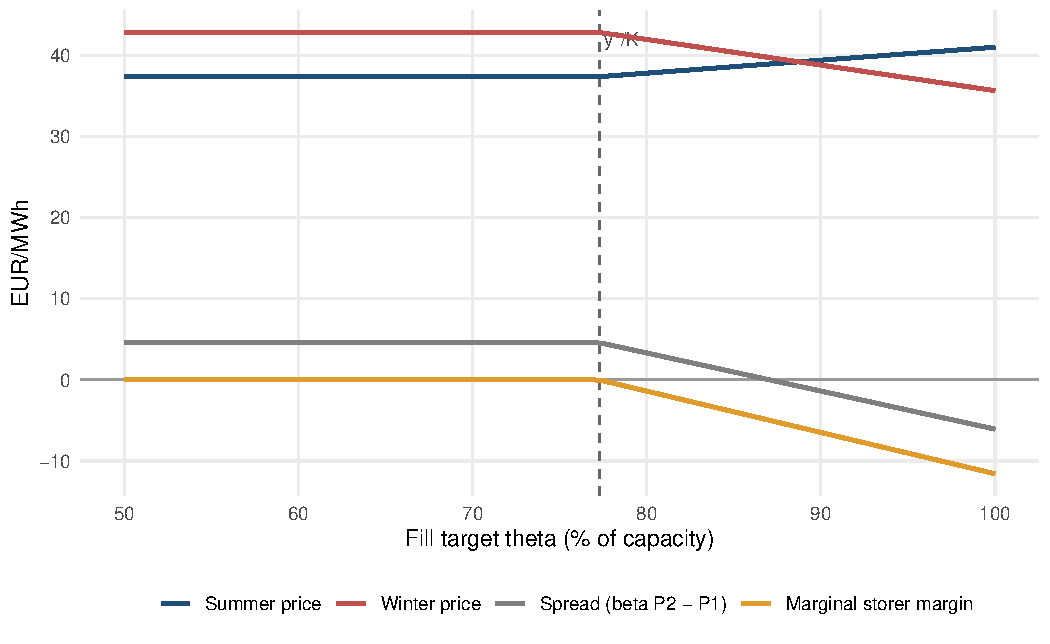
\includegraphics[width=0.85\textwidth]{fig1_prices_spread.pdf}
\caption{Summer and winter prices, the discounted spread and the marginal storer's margin as the target rises above the
competitive fill $y^*/K$.}\label{fig:prices}
\vspace{1em}
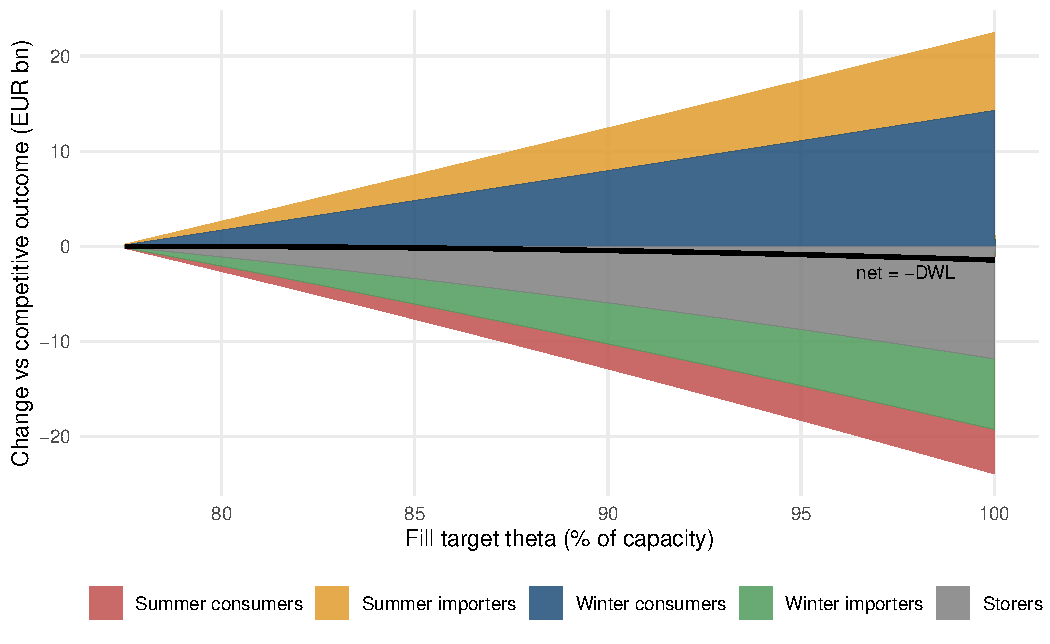
\includegraphics[width=0.85\textwidth]{fig2_incidence.pdf}
\caption{Incidence of an unfunded mandate relative to the competitive outcome, by target. Positive areas are gains, negative
areas losses; the black line is the net, $-\text{DWL}$.}\label{fig:incidence}
\end{figure}

\begin{figure}[p]
\centering
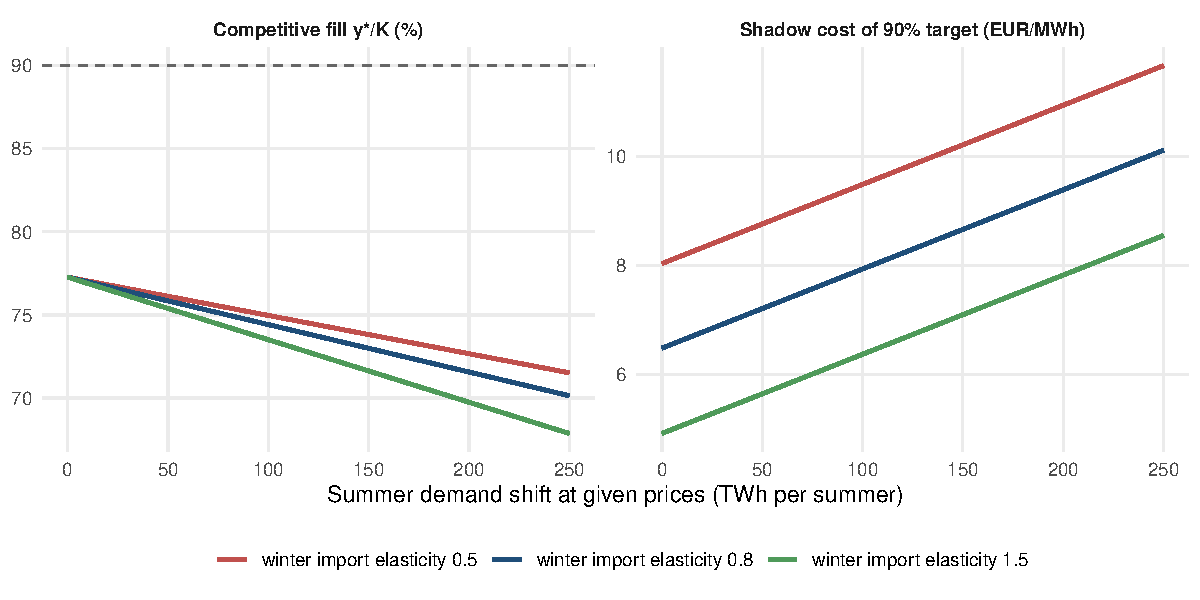
\includegraphics[width=0.95\textwidth]{fig3_seasonality_shift.pdf}
\caption{Distorted seasonality. Left: competitive fill as summer demand rises at given prices. Right: shadow cost $\nu$ of the 90\%
target. Each line recalibrates the no-storage spread so that the baseline fill is 77\%.}\label{fig:season}
\vspace{1em}
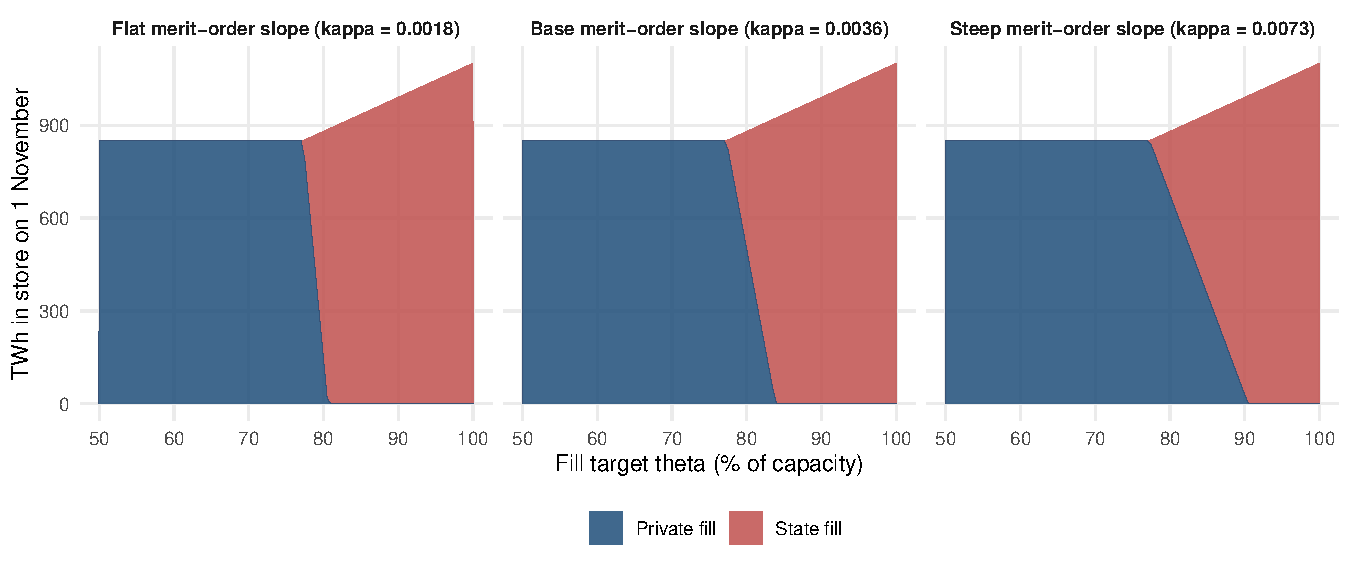
\includegraphics[width=\textwidth]{fig4_state_filling.pdf}
\caption{State filling as buyer of last resort: private and state fill on 1 November by target, for three slopes of the storage
merit order. Each mandated TWh crowds out $\sigma/\kappa$ TWh of private storage.}\label{fig:state}
\end{figure}

\section{How Step 1 generalises}\label{sec:extensions}

\paragraph{Step 2: uncertainty and the security benefit.} Let winter be normal or a crisis (cold spell, import disruption:
$A_2^H>A_2$ or an import cap $\bar M_2$) with probability $q$. Without frictions, the competitive $y^*$ is still efficient, now
with the expected spread in Proposition~\ref{prop:eq}. Adding one market failure that stops crisis scarcity being priced (a retail
or wholesale price cap $\bar P<\text{VoLL}$, non-price rationing, or expected state intervention) puts a wedge between the private
and social value of winter gas in the crisis state. The optimal target then solves
\[
\underbrace{\Lambda\,(\ybar-y^*)}_{\nu,\ \text{Step 1 cost}} \;=\; \underbrace{q\cdot\left(\text{VoLL}-\bar P\right)\cdot\Pr(\text{rationing}\mid\text{crisis},\ybar)}_{\text{marginal expected security benefit}} ,
\]
so the shadow cost derived here is exactly the price that the security benefit must cover. The terms $1-\omega_2$ (import
displacement) and $\bar M_2$ determine how much of the mandated gas is security-relevant.

\paragraph{Step 3: market power.} With $N$ storers competing in quantities, each internalises its own effect on both prices,
adding $-\sigma y_i$ to the first-order condition: storage is withheld relative to $y^*$, so a mandate can raise welfare even in
Step 1. With a dominant storer and a competitive fringe (the Baranes, Mirabel and Poudou (2014) structure, and the Rehden case
in our data) a uniform target binds asymmetrically, mostly on the dominant firm.

\paragraph{Step 4: the fill path and the deadline.} Split the summer into $J$ months with injection-rate limits. The single
arbitrage condition becomes a sequence $\beta^{j}P_2-P_{1j}-c_j-\kappa y=\mu_j+\nu$, where $\nu$ is the multiplier on the 1 November
target. Because the target is a stock at a date, $\nu$ enters every summer month and summer prices rise towards the deadline
when the target binds, which is the timing distortion in the ``distorted seasonality'' evidence.

\paragraph{Step 5: structural model.} Monthly periods, inventory as a state variable, demand shifters $A_t$ built from HDD, CDD and
gas-for-power, elastic LNG supply, several countries linked by interconnection with correlated shocks, and endogenous capacity
$K$. The Step 1 objects ($P_t^0$, $s_t$, $\kappa$, $\sigma$) become the season-level summary of that model, and the reduced form in
Section~\ref{sec:cs} is the first moment to match.

\appendix
\section{Proofs}

\paragraph{Lemma~\ref{lem:prices}.} Summer: $a_1+g_1(D_1+y)=A_1-b_1D_1$ gives $D_1=D_1^0-\frac{g_1}{b_1+g_1}y$, and substituting
into demand $P_1=A_1-b_1D_1^0+\frac{b_1g_1}{b_1+g_1}y=P_1^0+s_1y$. Winter is symmetric with $-y$.

\paragraph{Proposition~\ref{prop:eq}.} The price-taking first-order condition is $\beta P_2-P_1-c-\kappa y=\mu-\underline\mu$ with
multipliers on $y\le K$ and $y\ge 0$. Substituting Lemma~\ref{lem:prices}: $\Dz-\Lambda y=\mu-\underline\mu$. Rents:
$\Pi(y^*)=(c+\kappa y^*-c)y^*-\frac\kappa2y^{*2}=\frac\kappa2y^{*2}$.

\paragraph{Proposition~\ref{prop:eff}.} $\frac{d}{dy}(CS_1+PS_1)=-P_1(y)$ since one more unit stored removes one unit from the summer
market at the margin, valued at $P_1$; similarly $\frac{d}{dy}(CS_2+PS_2)=P_2(y)$. Adding $-C'(y)$ gives $W'$.

\paragraph{Propositions~\ref{prop:regimes}--\ref{prop:dwl}.}
$\Pi(\ybar)=(\Dz-\sigma\ybar)\ybar-\frac\kappa2\ybar^2\ge0\iff\Dz\ge(\sigma+\frac\kappa2)\ybar$. The inversion condition is
$\beta P_2-P_1=\Dz+c-\sigma\ybar<0$. $\text{DWL}=\int_{y^*}^{\ybar}(\Lambda y-\Dz)\,dy=\frac\Lambda2(\ybar^2-y^{*2})-\Lambda y^*G=\frac\Lambda2G^2$.
Surplus changes are trapezoids under linear curves, e.g.\ $\Delta CS_1=-\Delta P_1\frac{D_1^*+D_1(\ybar)}{2}$. Storers:
$\Pi(\ybar)-\Pi(y^*)=\Dz G-(\sigma+\frac\kappa2)(\ybar^2-y^{*2})$; with $\Dz=\Lambda y^*$ this equals $-\sigma Gy^*-(\sigma+\frac\kappa2)G^2$. The
five terms sum to $-\frac12\Lambda G^2$ (checked numerically in the R script).

\paragraph{Proposition~\ref{prop:tot}.} $\frac{d}{dy}PS_1=M_1s_1$ and $\frac{d}{dy}PS_2=-M_2s_2$; so $W_\alpha'(y^*)=-(1-\alpha)(s_1M_1^*-\beta s_2M_2^*)$,
positive iff $\beta s_2M_2^*>s_1M_1^*$. Concavity gives the closed form.

\paragraph{State filling.} The state fills the residual, so total storage is $\ybar$ and prices are $P_t(\ybar)$. The private
marginal facility stores iff $\Dz-\sigma\ybar\ge\kappa y_p$. The state's loss is
$(P_1+c-\beta P_2)z+\frac\kappa2(\ybar^2-y_p^2)$; with $P_1+c-\beta P_2=-\kappa y_p$ this is $\frac\kappa2z^2$.

\section*{References}
\begin{itemize}[label={}]
\item Baranes, E., Mirabel, F., and Poudou, J.-C. (2014). Natural gas storage and market power. \emph{Energy Economics}.
\item Ejarque, J. M. (2011). Evaluating the economic cost of natural gas strategic storage restrictions. \emph{Energy Economics}.
\end{itemize}

\end{document}
